\documentclass[tikz,border=16pt]{standalone}
\usepackage{tikz,amsmath,amssymb}
\usetikzlibrary{arrows.meta,calc}

\definecolor{CH}{HTML}{1f5c9e}   % blue   – hard primitive
\definecolor{CR}{HTML}{1a7870}   % teal   – reduction
\definecolor{CA}{HTML}{993c1d}   % coral  – adversary
\definecolor{CG}{HTML}{2a762a}   % green  – theorem / bound
\definecolor{CQ}{HTML}{6a3b90}   % purple – key question

\tikzset{
	ml/.style = {font=\tiny, fill=white, inner sep=1.5pt},
	ar/.style = {-{Stealth[scale=0.68]}, line width=0.78pt, #1},
	ar/.default = black,
}

\begin{document}
	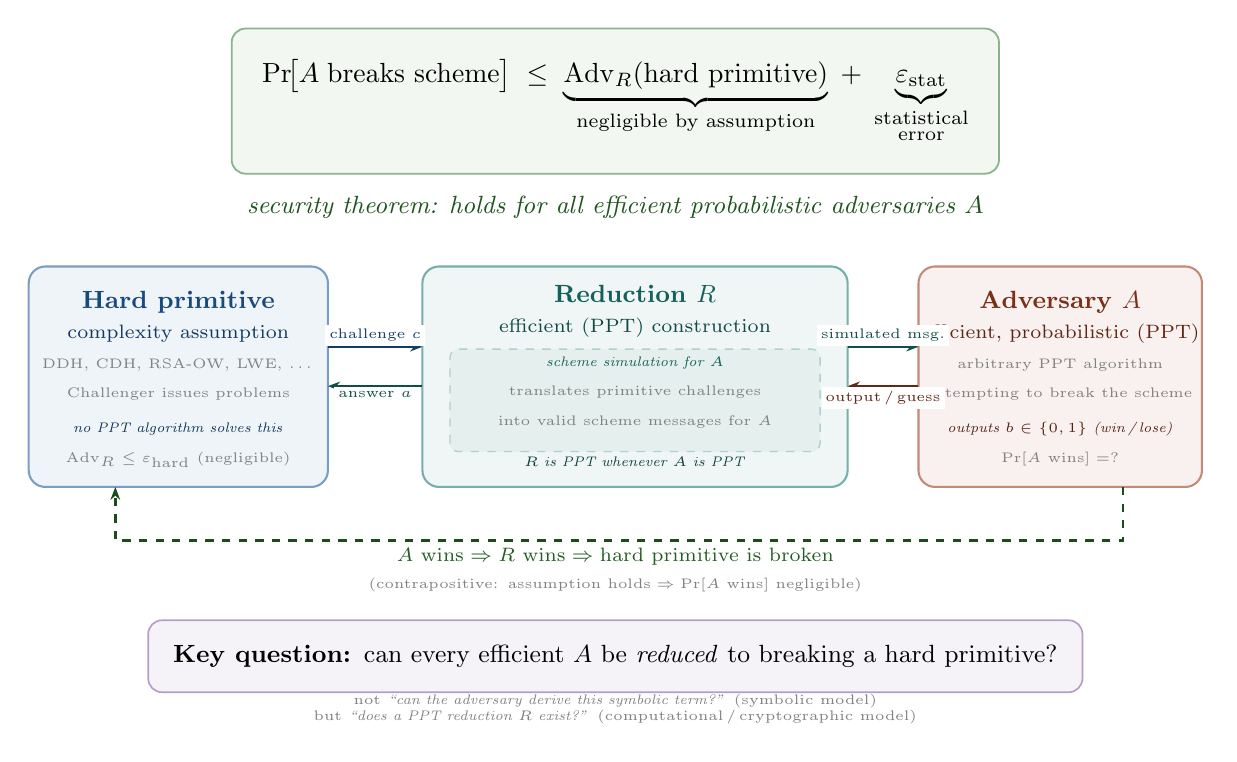
\begin{tikzpicture}
		
		%%═══════════════════════════════════════════════════════════════════
		%% THREE ACTOR BOXES   (all y = −1.4 … +1.4)
		%%   H : x = 0.3  … 4.1   center (2.2,  0)
		%%   R : x = 5.3  … 10.7  center (8.0,  0)
		%%   A : x = 11.6 … 15.2  center (13.4, 0)
		%%═══════════════════════════════════════════════════════════════════
		
		%% Hard Primitive ─────────────────────────────────────────────────
		\draw[draw=CH!60, fill=CH!7, rounded corners=6pt, line width=0.75pt]
		(0.3, -1.4) rectangle (4.1, 1.4);
		\node[font=\small\bfseries, color=CH!80!black] at (2.2,  0.95){Hard primitive};
		\node[font=\scriptsize,     color=CH!62!black] at (2.2,  0.55){complexity assumption};
		\node[font=\tiny,           color=gray]        at (2.2,  0.15){DDH, CDH, RSA-OW, LWE, \ldots};
		\node[font=\tiny,           color=gray]        at (2.2, -0.22){Challenger issues problems};
		\node[font=\tiny,           color=CH!55!black] at (2.2, -0.66){\textit{no PPT algorithm solves this}};
		\node[font=\tiny,           color=gray]        at (2.2, -1.05)%
		{$\mathrm{Adv}_{R} \leq \varepsilon_{\mathrm{hard}}$ (negligible)};
		
		%% Reduction ───────────────────────────────────────────────────────
		\draw[draw=CR!60, fill=CR!7, rounded corners=6pt, line width=0.75pt]
		(5.3, -1.4) rectangle (10.7, 1.4);
		%% inner dashed sub-box: scheme simulation
		\draw[draw=CR!35, fill=CR!12, dashed, rounded corners=3pt, line width=0.5pt]
		(5.65, -0.95) rectangle (10.35, 0.35);
		\node[font=\small\bfseries, color=CR!80!black] at (8.0,  1.05){Reduction $R$};
		\node[font=\scriptsize,     color=CR!62!black] at (8.0,  0.62){efficient (PPT) construction};
		\node[font=\tiny,           color=CR!80!black] at (8.0,  0.17){\textit{scheme simulation for $A$}};
		\node[font=\tiny,           color=gray]        at (8.0, -0.20){translates primitive challenges};
		\node[font=\tiny,           color=gray]        at (8.0, -0.58){into valid scheme messages for $A$};
		\node[font=\tiny,           color=CR!55!black] at (8.0, -1.08)%
		{\textit{$R$ is PPT whenever $A$ is PPT}};
		
		%% Adversary ───────────────────────────────────────────────────────
		\draw[draw=CA!60, fill=CA!7, rounded corners=6pt, line width=0.75pt]
		(11.6, -1.4) rectangle (15.2, 1.4);
		\node[font=\small\bfseries, color=CA!80!black] at (13.4,  0.95){Adversary $A$};
		\node[font=\scriptsize,     color=CA!62!black] at (13.4,  0.55){efficient, probabilistic (PPT)};
		\node[font=\tiny,           color=gray]        at (13.4,  0.15){arbitrary PPT algorithm};
		\node[font=\tiny,           color=gray]        at (13.4, -0.22){attempting to break the scheme};
		\node[font=\tiny,           color=CA!55!black] at (13.4, -0.66)%
		{\textit{outputs $b \in \{0,1\}$ (win\,/\,lose)}};
		\node[font=\tiny,           color=gray]        at (13.4, -1.05)%
		{$\Pr[A\text{ wins}] = ?$};
		
		%%═══════════════════════════════════════════════════════════════════
		%% INTERACTION ARROWS
		%%═══════════════════════════════════════════════════════════════════
		
		%% H ↔ R
		\draw[ar=CH!65!black] (4.1,  0.38) --
		node[ml, above]{challenge $c$} (5.3,  0.38);
		\draw[ar=CR!65!black] (5.3, -0.12) --
		node[ml, below]{answer $a$}    (4.1, -0.12);
		
		%% R ↔ A
		\draw[ar=CR!65!black] (10.7,  0.38) --
		node[ml, above]{simulated msg.} (11.6,  0.38);
		\draw[ar=CA!65!black] (11.6, -0.12) --
		node[ml, below]{output\,/\,guess}  (10.7, -0.12);
		
		%%═══════════════════════════════════════════════════════════════════
		%% IMPLICATION ARC  A wins → R wins → primitive broken
		%%═══════════════════════════════════════════════════════════════════
		\draw[ar=CG!65!black, dashed, line width=0.85pt]
		(14.2, -1.40) -- (14.2, -2.08) -- (1.4, -2.08) -- (1.4, -1.40);
		\node[font=\scriptsize, color=CG!80!black] at (7.75, -2.28)
		{$A$ wins\;$\Rightarrow$\;$R$ wins\;%
			$\Rightarrow$\;hard primitive is broken};
		\node[font=\tiny, color=gray] at (7.75, -2.65)
		{(contrapositive:\enspace assumption holds\;%
			$\Rightarrow$\;$\Pr[A\text{ wins}]$ negligible)};
		
		%%═══════════════════════════════════════════════════════════════════
		%% THEOREM BOX  (top)
		%%═══════════════════════════════════════════════════════════════════
		\node[draw=CG!55, fill=CG!6, rounded corners=5pt, line width=0.65pt,
		inner sep=11pt, font=\normalsize] at (7.75, 3.50) {%
			$\displaystyle
			\Pr\!\bigl[A\;\text{breaks scheme}\bigr]
			\;\leq\;
			\underbrace{%
				\mathrm{Adv}_{R}(\text{hard primitive})%
			}_{\text{negligible by assumption}}
			\;+\;
			\underbrace{%
				\varepsilon_{\mathrm{stat}}%
			}_{\substack{\text{statistical}\\\text{error}}}$};
		\node[font=\small\itshape, color=CG!72!black] at (7.75, 2.15)
		{security theorem: holds for all efficient probabilistic adversaries $A$};
		
		%%═══════════════════════════════════════════════════════════════════
		%% KEY QUESTION BOX  (bottom)
		%%═══════════════════════════════════════════════════════════════════
		\node[draw=CQ!50, fill=CQ!6, rounded corners=5pt, line width=0.60pt,
		inner sep=9pt, font=\small] at (7.75, -3.55)
		{\textbf{Key question:}\enspace
			can every efficient $A$ be \emph{reduced} to breaking a hard primitive?};
		
		\node[font=\tiny, color=gray, align=center] at (7.75, -4.22)
		{not \textit{``can the adversary derive this symbolic term?''}%
			\enspace(symbolic model)\\
			but \textit{``does a PPT reduction $R$ exist?''}%
			\enspace(computational\,/\,cryptographic model)};
		
	\end{tikzpicture}
\end{document}